\documentclass{article}

% Paquetes para mejor apariencia y personalización
\usepackage{amsmath}
\numberwithin{equation}{section}
\usepackage[utf8]{inputenc}  % Codificación de caracteres
\usepackage{graphicx}        % Incluir imágenes
\usepackage{imakeidx}
%\usepackage{amsmath, amssymb, amsfonts}
%\usepackage{hyperref}
\makeindex[options=-c, intoc]


\title{MÉTODOS DE DETERMINACIÓN DE ÓRBITAS A PARTIR DE OBSERVACIONES}   % Título del artículo
\author{
    Víctor Ávila Camargo, José Ignacio Miguel Rodríguez, Javier Zaragozano Calvo
}
\date{\today}  % Fecha del artículo, por defecto pone la fecha actual.

\begin{document}

% Generar la portada
\maketitle
%\includegraphics[width=1\textwidth]{portada.jpg}
\newpage

\tableofcontents

\newpage

\begin{abstract}
    En este artículo se abordarán varios métodos para determinar 
    las órbitas de cuerpos celestes a partir de observaciones 
    proporcionadas por la NASA.
\end{abstract}
\newpage
\section{Introducción} %Motivación del problema
\index{Introducción}
Hoy en día y desde hace ya un tiempo, 
varios exoplanetas son descubiertos a diario, cada uno con sus propias características. 
Para terminar de caracterizarlos por completo, es necesario 
hacer un estudio de cómo es su órbita. Esto es importante porque estudiando su órbita podemos recabar algunos 
datos que de otro modo sería imposible. 
Por ejemplo, podemos ver si el exoplaneta se encuentra en la zona habitable 
de su estrella o no, viendo qué tan grande es el periodo de su 
órbita. \\

Sin embargo, tomar una medida de su posición cada día sería 
algo tremendamente ineficiente. Es por eso que antiguos 
matemáticos y físicos desarrollaron algunos métodos para 
determinar su órbita de manera preliminar a partir de, generalmente, 
tres medidas. Algunos de estos métodos son el método de 
Gauss o el método de Gibbs. \\

Estos métodos han logrado varios hitos bastante importantes 
en la historia de la mecánica celeste. Uno de estos logros 
y quizás el más importante fue la determinación de la órbita 
del planeta enano Ceres. Este planeta enano fue descubierto 
el 1 de enero de 1801 por el astrónomo italiano Giuseppe Piazzi ($1746-1826$). 
Sin embargo, debido a su rápido movimiento, pronto le perdieron 
de vista y ahí es cuando aparece la gran aportación del matemático Carl Friedrich Gauss ($1777-1855$), 
que, con su método, calculó la órbita de Ceres a partir de 
las pocas observaciones que había de él en la época y, gracias 
a su alta precisión, pudieron volver a localizarle. \\

Una vez motivado el esfuerzo de dedicarle un artículo a los 
método de determinación de órbitas, vamos a comenzar desarrollando 
el aspecto más teórico de los dos métodos en los que nos 
vamos a centrar: El método de Gauss y el método de Gibbs.
\section{Método de Gibbs}
\index{Método de Gibbs}
Para este método es necesario conocer la posición de un cuerpo 
respecto a la Tierra en 3 instantes de tiempo distintos, 
$t_{1}$, $t_{2}$ y $t_{3}$. A partir de estas tres posiciones, 
podremos obtener las velocidades $\overrightarrow{v_{1}}$, 
$\overrightarrow{v_{2}}$ y $\overrightarrow{v_{3}}$ suponiendo 
que nos encontramos en una órbita de dos cuerpos. La solución a 
este problema la obtuvo el americano J.W. Gibbs ($1839-1903$) 
usando simplemente un análisis vectorial. A continuación, 
entraremos más en detalle sobre cómo se deduce este método.
\subsection{Deducción del método de Gibbs}
Sabemos que por la conservación del momento angular, 
las posiciones de un cuerpo que orbita alrededor de otro se encuentran todas 
en el mismo plano. Entonces, partiendo de nuestras tres posiciones 
obtenidas en tres tiempos distintos, podemos calcular el 
vector unitario de $\overrightarrow{r_{1}}$ y otro vector 
unitario que sea resultado del producto vectorial de $r_{2}$ y 
$r_{3}$ del siguiente modo: 
\begin{align*}
    &\hat{u}_{r1}=\frac{\overrightarrow{r_{1}}}{r_{1}} \\
    &\hat{C}_{23}=\frac{\overrightarrow{r_{2}}\times \overrightarrow{r_{3}}}{\left\lVert \overrightarrow{r_{2}}\times \overrightarrow{r_{3}} \right\rVert }  
\end{align*}
Como $\overrightarrow{r_{1}}$, $\overrightarrow{r_{2}}$ y 
$\overrightarrow{r_{3}}$ están en el mismo plano, entonces: 
\begin{equation*}
    \hat{u}_{r1}\cdot \hat{C}_{23}=0
\end{equation*}
Además, como se ve en la siguiente figura, nosotros podemos 
expresar $\overrightarrow{r_{2}}$ como una combinación lineal 
de $\overrightarrow{r_{1}}$ y $\overrightarrow{r_{3}}$: 
\begin{equation}
    \overrightarrow{r_{2}}=\alpha \overrightarrow{r_{1}}+\beta \overrightarrow{r_{3}}
\end{equation}
\begin{figure}[h]
    \centering
    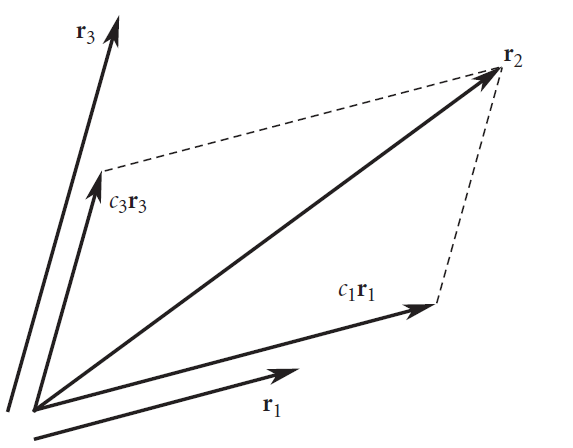
\includegraphics[width=0.6\textwidth]{a.png}
    \caption{Demostración de la ecuación 2.1 (Créditos 
    HowardD. Curtis)}
\end{figure} \\

Una vez tenemos estas consideraciones en mente ya podemos 
empezar a calcular las distintas velocidades. \\

Para calcular las velocidades vamos a partir de la siguiente 
fórmula: 
\begin{equation}
    \overrightarrow{v}\times \overrightarrow{h}=\mu\left(\frac{\overrightarrow{r}}{r}+\overrightarrow{e}\right) 
\end{equation}
Donde $\overrightarrow{h}$ es el momento angular y 
$\overrightarrow{e}$ es el vector excentricidad. Para despejar 
$\overrightarrow{v}$ vamos a multiplicar vectorialmente a ambos 
lados por $\overrightarrow{h}$. Entonces, centrándonos de momento 
en lado izquierdo de la ecuación, obtenemos: 
\begin{equation*}
    \overrightarrow{h}\times(\overrightarrow{v}\times\overrightarrow{h})
\end{equation*}
Para continuar vamos a aplicar la siguiente propiedad del 
triple producto vectorial: $\overrightarrow{A}\times(\overrightarrow{B}\times\overrightarrow{C})
=(\overrightarrow{A}\cdot\overrightarrow{C})\overrightarrow{B}-(\overrightarrow{A}\cdot\overrightarrow{B})\overrightarrow{C}$
y obtenemos lo siguiente: 
\begin{equation*}
    \overrightarrow{h}\times(\overrightarrow{v}\times\overrightarrow{h})=(\overrightarrow{h}\cdot\overrightarrow{h})\overrightarrow{v}-(\overrightarrow{v}\cdot\overrightarrow{h})\overrightarrow{h}
\end{equation*}
Pero como $\overrightarrow{h}\cdot\overrightarrow{h}=h^{2}$ y 
$\overrightarrow{v}\perp\overrightarrow{h}$ obtenemos: 
\begin{equation*}
    \overrightarrow{h}\times(\overrightarrow{v}\times\overrightarrow{h})=h^{2}\overrightarrow{v}
\end{equation*}
Y nuestra ecuación 2.2 queda de la siguiente manera:
\begin{equation}
    \overrightarrow{v}=\frac{\mu}{h^{2}}\left(\frac{\overrightarrow{h}\times\overrightarrow{r}}{r}+\overrightarrow{h}\times\overrightarrow{e}\right)
\end{equation}
Cabe destacar que, en el sistema perifocal, el vector unidad 
$\hat{p}$ tiene la misma dirección que el vector 
de la excentricidad y el vector $\hat{w}$ es perpendicular 
al plano de la órbita en la dirección de $\overrightarrow{h}$. Por 
lo que, en el sistema perifocal, nuestra ecuación se transforma en: 
\begin{equation}
    \overrightarrow{v}=\frac{\mu}{h^{2}}\left(\frac{h\hat{w}\times\overrightarrow{r}}{r}+h\hat{w}\times e\hat{p}\right)=\frac{\mu}{h}\left[\frac{\hat{w}\times\overrightarrow{r}}{r}+e(\hat{w}\times\hat{p})\right]
\end{equation}
Como $\hat{w}$ y $\hat{p}$ son 2 vectores 
de la base en el sistema perifocal, entonces su producto 
vectorial será el tercer vector de la base ($\hat{q}$). 
Así que esto hace que nuestra ecuación se reduzca a: 
\begin{equation}
    \overrightarrow{v}=\frac{\mu}{h}\left(\frac{\hat{w}\times\overrightarrow{r}}{r}+e\hat{q}\right)
\end{equation}
Este es un resultado muy importante porque nos marca nuestro 
camino a seguir. Necesitamos encontrar una forma de obtener 
los vectores y magnitudes $\hat{p}$, $\hat{q}$, 
$\hat{w}$, $h$ y $e$ a partir de nuestros tres 
vectores de posiciones y así poder aplicar la fórmula 2.5. \\

Como nuestros tres vectores de posición son parte de una 
órbita, podemos multiplicar a nuestra ecuación 2.1 por el 
vector excentricidad y obtener: 
\begin{equation*}
    \overrightarrow{r_{2}}\cdot\overrightarrow{e}=\alpha\overrightarrow{r_{1}}\cdot\overrightarrow{e}+\beta\overrightarrow{r_{3}}\cdot\overrightarrow{e}
\end{equation*} 
Estos productos escalares dan como resultado: 
\begin{equation}
    \overrightarrow{r_{i}}\cdot\overrightarrow{e}=\frac{h^{2}}{\mu}-r_{i} 
\end{equation}
Por lo que si lo sustituimos todo al final llegamos a:
\begin{equation}
    \frac{h^{2}}{\mu}-r_{2}=\alpha\left(\frac{h^{2}}{\mu}-r_{1}\right)+\beta\left(\frac{h^{2}}{\mu}-r_{3}\right)
\end{equation}
Ahora, nuestro objetivo es eliminar los coeficientes $\alpha$ 
y $\beta$ por lo que, para ello, vamos a multiplicar vectorialmente 
a nuestra ecuación 2.1 por $\overrightarrow{r_{1}}$ y 
por $\overrightarrow{r_{3}}$ obteniendo así:
\begin{align*}
    &\overrightarrow{r_{2}}\times\overrightarrow{r_1}=\beta(\overrightarrow{r_{3}}\times\overrightarrow{r_{1}})   &\overrightarrow{r_{2}}\times\overrightarrow{r_3}=-\alpha(\overrightarrow{r_{3}}\times\overrightarrow{r_{1}})
\end{align*}
Con este resultado en mente, si multiplicamos a nuestra ecuación 
2.7 por el producto vectorial de $\overrightarrow{r_3}$ y 
$\overrightarrow{r_1}$ vamos a obtener:
\begin{equation*}
    \frac{h^{2}}{\mu}(\overrightarrow{r_{3}}\times\overrightarrow{r_{1}})-r_{2}(\overrightarrow{r_{3}}\times\overrightarrow{r_{1}})=-(\overrightarrow{r_{2}}\times\overrightarrow{r_{3}})\left(\frac{h^{2}}{\mu}-r_{1} \right)+(\overrightarrow{r_{2}}\times\overrightarrow{r_{1}})\left(\frac{h^{2}}{\mu}-r_{3} \right)
\end{equation*}
Gracias a esto, hemos podido eliminar los coeficientes 
$\alpha$ y $\beta$. Si agrupamos términos al final obtenemos: 
\begin{equation*}
    \frac{h^{2}}{\mu}(\overrightarrow{r_{1}}\times\overrightarrow{r_{2}}+\overrightarrow{r_{2}}\times\overrightarrow{r_{3}}+\overrightarrow{r_{3}}\times\overrightarrow{r_{1}})=r_{1}(\overrightarrow{r_{2}}\times\overrightarrow{r_{3}})+r_{2}(\overrightarrow{r_{3}}\times\overrightarrow{r_{1}})+r_{3}(\overrightarrow{r_{1}}\times\overrightarrow{r_{2}}) 
\end{equation*}
Para poner esta ecuación de un modo más simple, vamos a llamar 
al paréntesis de la izquierda $\overrightarrow{D}$ y a la 
parte de la derecha $\overrightarrow{N}$. Entonces: 
\begin{equation}
    \overrightarrow{N}=\frac{h^{2}}{\mu}\overrightarrow{D} 
\end{equation}
Poniendo esta ecuación en función de los módulos N y D (esencialmente 
es la misma ecuación), podemos despejar h y obtener: 
\begin{equation}
    h=\sqrt{\mu\frac{N}{D}}
\end{equation}
Como N y D dependen solo de los vectores de posición ya hemos 
conseguido uno de nuestros objetivos, el de obtener h a partir 
de los vectores de posición. Además, como todos los vectores son 
coplanarios, todos sus productos vectoriales van a ser perpendiculares 
al plano de la órbita pudiendo definir: 
\begin{equation}
    \hat{w}=\frac{\overrightarrow{D}}{D} 
\end{equation}
Ya tenemos $\hat{w}$ en función de los vectores de posición. Sin 
embargo, también necesitamos hacer lo mismo para $\hat{q}$.
Si recordamos, $\hat{q}$ lo podemos escribir como: 
\begin{equation*}
    \hat{q}=\hat{w}\times\hat{p}=\frac{1}{De}(\overrightarrow{D}\times\overrightarrow{e}) 
\end{equation*}
Sustituyendo el valor de $\overrightarrow{D}$ obtenemos: 
\begin{equation*}
    \hat{q}=\hat{w}\times\hat{p}=\frac{1}{De}[(\overrightarrow{r_{1}}\times\overrightarrow{r_{2}})\times\overrightarrow{e}+(\overrightarrow{r_{2}}\times\overrightarrow{r_{3}})\times\overrightarrow{e}+(\overrightarrow{r_{3}}\times\overrightarrow{r_{1}})\times\overrightarrow{e}]
\end{equation*}
Si aplicamos la ya mencionada propiedad del producto 
vectorial triple y teniendo en cuenta la ecuación 2.7, 
al final obtenemos: 
\begin{equation}
    \hat{q}=\frac{1}{De}\overrightarrow{S} 
\end{equation}
Donde $\overrightarrow{S}=\overrightarrow{r_{1}}(r_{2}-r_{3})+\overrightarrow{r_{2}}(r_{3}-r_{1})+\overrightarrow{r_{3}}(r_{1}-r_{2})$. 
Finalmente, si sustituimos de vuelta en nuestra ecuación 2.5 tenemos: 
\begin{equation*}
    \overrightarrow{v}=\frac{\mu}{\sqrt{\mu\frac{N}{D}}}\left[\frac{\frac{\overrightarrow{D}}{D}\times\overrightarrow{r}}{r}+e\left(\frac{1}{De}\overrightarrow{S}\right) \right] 
\end{equation*}
La cual, tras simplificar, se transforma en: 
\begin{equation}
    \overrightarrow{v}=\sqrt{\frac{\mu}{ND}}\left(\frac{\overrightarrow{D}\times\overrightarrow{r}}{r}+\overrightarrow{S}\right) 
\end{equation}
Ya tenemos todos los elementos de esta ecuación en función de 
nuestros tres vectores de posiciones iniciales, por lo que 
ya somos capaces de determinar la órbita de cualquier 
objeto celeste (suponiendo que estamos en un problema de dos 
cuerpos) a partir de tres medidas iniciales de su posición. 
\subsection{Resumen}
Para finalizar, vamos a poner las fórmulas más importantes 
de este desarrollo que se usarán en el algoritmo de este 
método que será mostrado en secciones posteriores:
\begin{align*}
    &\overrightarrow{S}=\overrightarrow{r_{1}}(r_{2}-r_{3})+\overrightarrow{r_{2}}(r_{3}-r_{1})+\overrightarrow{r_{3}}(r_{1}-r_{2}) \\
    &\overrightarrow{D}=\overrightarrow{r_{1}}\times\overrightarrow{r_{2}}+\overrightarrow{r_{2}}\times\overrightarrow{r_{3}}+\overrightarrow{r_{3}}\times\overrightarrow{r_{1}} \\
    &\overrightarrow{N}=r_{1}(\overrightarrow{r_{2}}\times\overrightarrow{r_{3}})+r_{2}(\overrightarrow{r_{3}}\times\overrightarrow{r_{1}})+r_{3}(\overrightarrow{r_{1}}\times\overrightarrow{r_{2}}) \\
    &\overrightarrow{v}=\sqrt{\frac{\mu}{ND}}\left(\frac{\overrightarrow{D}\times\overrightarrow{r}}{r}+\overrightarrow{S}\right) 
\end{align*}
\section{Método de Gauss}
\index{Método de Gauss}

El siguiente método para la determinación preliminar de órbitas es el método de Gauss. Al igual que en el de Gibbs, necesitamos tres observaciones en tres tiempos distintos para poder comenzar con el procedimiento, pero en esta ocasión necesitamos datos distintos.\par

El método de Gauss está basado en la determinación de órbitas a partir de \textbf{ángulos}. En el método anterior precisábamos de la posición y velocidad del cuerpo en tres momentos distintos, ahora partimos de dos ángulos en tres instantes de tiempo, estos son la ascensión recta $\alpha$ y la declinación $\delta$.\par

\begin{figure}[h]
    \centering
    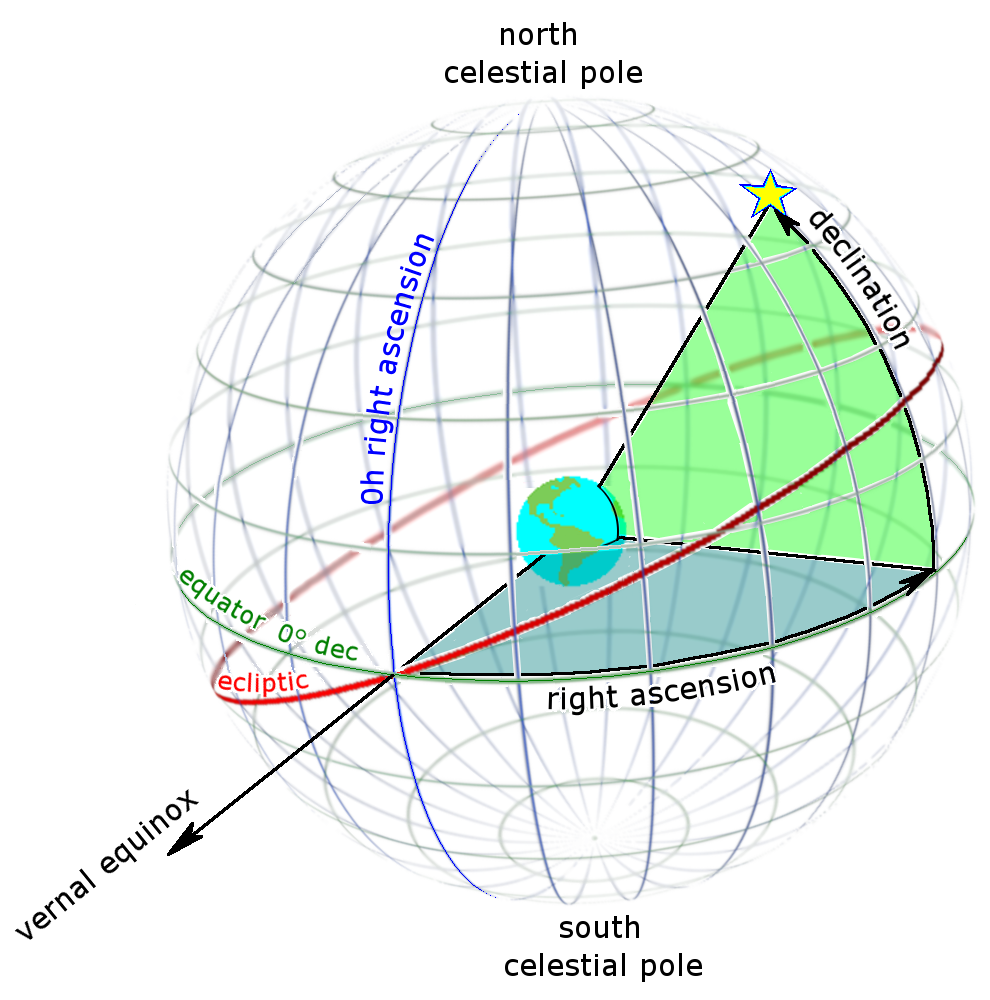
\includegraphics[width=0.55\textwidth]{ARyD.png}
    \caption{Ascensión Recta y Declinación (Créditos 
    Wikipedia)}
\end{figure} 
Esto es especialmente útil cuando no tenemos información de nuestra distancia hasta el cuerpo o solo podemos observarlo con instrumentos que no nos dan esa información. Así pues, usando estos ángulos que sí podemos conocer en función del punto de observación terrestre, podemos obtener una vista preliminar de las órbitas de los objetos celestes que nos interesen.\par

\subsection{Desarrollo del método}

Dado que la deducción matemática no es trivial y para ayudar a la comprensión del lector, explicaremos este método de una forma secuencial e iremos desarrollándolo a modo de algoritmo mientras exponemos las ecuaciones necesarias en cada etapa del mismo.\par

Para comenzar con el método necesitamos partir de algunos datos. Estos son:

\begin{itemize}
    \item Tiempos de observación: $t_1$, $t_2$, $t_3$.
    \item Vectores de posición del observador en dichos tiempos: $\overrightarrow{R_1}$, $\overrightarrow{R_2}$, $\overrightarrow{R_3}$.
            \item Vectores unitarios de dirección topocéntricos: $\hat{\mathbf{\varrho}}_1$, $\hat{\mathbf{\varrho}}_2$, $\hat{\mathbf{\varrho}}_3$. Estos apuntan desde el observador hacia el cuerpo y se pueden obtener antes de empezar midiendo $\alpha$ y $\delta$ del cuerpo en cada tiempo de observación.
\end{itemize}

\begin{figure}[h]
    \centering
    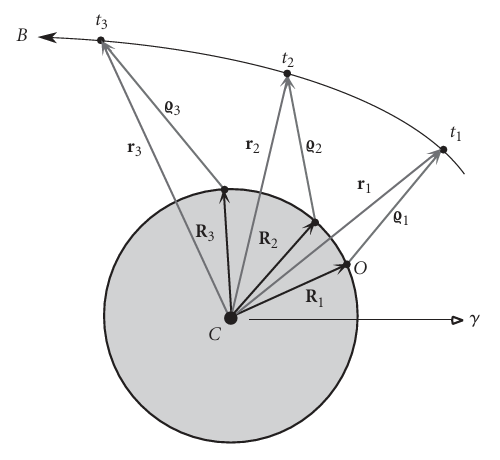
\includegraphics[width=0.65\textwidth]{entra.png}
    \caption{Esquema vectorial de los datos de entrada para el método de Gauss, donde C es el centro de atracción, O el observador y B el cuerpo en órbita. (Créditos 
    HowardD. Curtis)}
\end{figure} 
\newpage
Antes de pasar a ver los pasos, vamos a plantear el problema para ver cómo luego lo resolvemos. Según vemos en la figura 3, los vectores $\overrightarrow{r_i}$ son desconocidos a la vez que necesarios para determinar la órbita del cuerpo. Sin embargo podemos escribir estas tres ecuaciones:\par

\begin{align}
    \overrightarrow{r_1} = \overrightarrow{R_1} + \varrho_1 \hat{\varrho_1} \\
    \overrightarrow{r_2} = \overrightarrow{R_2} + \varrho_2 \hat{\varrho_2} \\
    \overrightarrow{r_3} = \overrightarrow{R_3} + \varrho_3 \hat{\varrho_3}
\end{align}

Al ser ecuaciones vectoriales disponemos de nueve ecuaciones escalares y de 12 incógnitas (las tres componentes de cada vector de posición, más los tres módulos de las direcciones topocéntricas). Como vemos, necesitamos más ecuaciones para poder sacar una solución al sistema.\par

Si seguimos buscando recursos, podemos echar mano de una de las asunciones que hacíamos en el método de Gibbs, en concreto, de que los tres vectores $\overrightarrow{r_i}$ deben pertenecer al mismo plano por la conservación del momento angular (podemos expresar uno de ellos en función de los otros dos). De esto sacamos:

\begin{equation}
    \overrightarrow{r_2} = c_1\cdot\overrightarrow{r_1} + c_3\cdot\overrightarrow{r_3}
\end{equation}

Con esta nueva ecuación vectorial introducimos 2 nuevas incógnitas, los coeficientes $c_1$ y $c_3$. Si hacemos un recuento ahora tenemos 12 ecuaciones para 14 incógnitas. Cada vez estamos más cerca de poder resolver el sistema.\par

Si continuamos buscando ecuaciones que nos ayuden, podemos aprovecharnos de otra consecuencia de la ecuación de movimiento del problema de los dos cuerpos, y es que el vector de estados (que contiene a $\overrightarrow{r}$ y $\overrightarrow{v}$) del cuerpo en órbita se puede expresar como el vector de estados en cualquier tiempo dado mediante los \textbf{coeficientes de Lagrange} de la siguiente forma:

\begin{align}
    \overrightarrow{r_1} = f_1\cdot\overrightarrow{r_2} + g_1\cdot\overrightarrow{v_2} \\
    \overrightarrow{r_3} = f_3\cdot\overrightarrow{r_2} + g_3\cdot\overrightarrow{v_2}
\end{align}

donde $f_i$ y $g_i$ son los coeficientes de Lagrange evaluados en el tiempo $t_i$. Además, si los intervalos de tiempo son lo suficientemente pequeños se puede comprobar que las funciones $f$ y $g$ dependen solo de la distancia al centro de atracción, en nuestro caso, trabajamos con $r_2$. Por tanto, estas dos ecuaciones vectoriales nos añaden 6 ecuaciones escalares y 4 incógnitas (las tres componentes de $\overrightarrow{v_2}$ y la magnitud $r_2$). Si sumamos esto al sistema que ya teníamos, obtenemos un total de 18 ecuaciones escalares para una suma de 18 incógnitas. Por fin el problema está bien preparado para proponer una solución. Antes de empezar, mantengamos en mente que el objetivo será obtener el vector de estados en el instante de tiempo intermedio $t_2$, es decir, $\overrightarrow{r_2}$ y $\overrightarrow{v_2}$, pues con esto determinado podremos obtener los elementos orbitales de la trayectoria de nuestro cuerpo.\\

Visto todo esto, procedamos con los pasos para conseguir nuestro objetivo:\\

\noindent\textbf{1. Obtener intervalos de tiempo}

Primero definimos los intervalos de tiempo $\tau_1$, $\tau_3$ y $\tau$ de la siguiente forma:

\begin{align}
    \tau_1= t_1-t_2 \\
    \tau_3= t_3-t_2 \\
    \tau= \tau_3-\tau_1
\end{align}

Estos son los intervalos de tiempo entre las observaciones y el intervalo de tiempo total. Como explicamos antes, si los intervalos son suficientemente cortos, podremos aprovechar las propiedades de los coeficientes de Lagrange.\\

\noindent\textbf{2. Obtener productos vectoriales $p_i$}

Para poder resolver el sistema de ecuaciones necesitaremos calcular los siguientes productos vectoriales para posteriormente simplificar los productos escalares triples.

\begin{align}
    \overrightarrow{p_1}=\hat{\varrho_2}\times\hat{\varrho_3} \hspace{1.5cm} & \overrightarrow{p_2}=\hat{\varrho_1}\times\hat{\varrho_3} \hspace{1cm} & \overrightarrow{p_3}=\hat{\varrho_1}\times\hat{\varrho_3}
\end{align}

\noindent\textbf{3. Obtener productos escalares triples $D$}

Haciendo uso de los productos vectoriales calculados anteriormente, vamos a calcular las siguientes cantidades escalares:

\begin{equation}
    D_0=\hat{\varrho_1}\cdot\overrightarrow{p_1}
\end{equation}

\begin{equation}
\begin{array}{ccc}
D_{11} = \overrightarrow{R_1} \cdot \overrightarrow{p_1} & D_{12} = \overrightarrow{R_1} \cdot \overrightarrow{p_2} & D_{13} = \overrightarrow{R_1} \cdot \overrightarrow{p_3} \\
D_{21} = \overrightarrow{R_2} \cdot \overrightarrow{p_1} & D_{22} = \overrightarrow{R_2} \cdot \overrightarrow{p_2} & D_{23} = \overrightarrow{R_2} \cdot \overrightarrow{p_3} \\
D_{31} = \overrightarrow{R_3} \cdot \overrightarrow{p_1} & D_{32} = \overrightarrow{R_3} \cdot \overrightarrow{p_2} & D_{33} = \overrightarrow{R_3} \cdot \overrightarrow{p_3}
\end{array}
\end{equation}

Estas magnitudes son necesarias ya que en el desarrollo del sistema, nos vamos a topar con expresiones para los $\varrho_i$ y el resto de incógnitas en función de estos productos. Tenerlos calculados nos permite agilizar el proceso.\\

\noindent\textbf{4. Obtener expresiones para las longitudes $\varrho_i$}

Este paso precisa de haber hecho un desarrollo de nuestras ecuaciones del sistema empleando cálculo vectorial. Para evitar atascarnos despejando ecuaciones, vamos a mostrar el procedimiento y sus resultados, dejando como tarea pendiente demostrar las ecuaciones que vamos a presentar.\par

Partiremos de la ecuación 5.4 resolviendo para $c_1$ y $c_3$:

\begin{equation}
    c_1 = \frac{(\overrightarrow{r_2} \times \overrightarrow{r_3}) \cdot (\overrightarrow{r_1} \times \overrightarrow{r_3})}{\|\overrightarrow{r_1} \times \overrightarrow{r_3}\|^2}
\end{equation}

\begin{equation}
    c_3 = \frac{(\overrightarrow{r_2} \times \overrightarrow{r_1}) \cdot (\overrightarrow{r_3} \times \overrightarrow{r_1})}{\|\overrightarrow{r_1} \times \overrightarrow{r_3}\|^2}
\end{equation}

Si ahora utilizamos las ecuaciones 5.5 y 5.6, que expresan $\overrightarrow{r_1}$ y $\overrightarrow{r_3}$ en función de los coeficientes de Lagrange, entonces podemos sustituir en estas ecuaciones para $c_1$ y $c_3$, obteniendo:

\begin{equation}
c_1 = \frac{g_3}{f_{1}g_3 - f_{3}g_1}
\end{equation}

\begin{equation}
c_3 = -\frac{g_1}{f_{1}g_3 - f_{3}g_1}
\end{equation}

Hemos conseguido expresarlos solo en función de estos coeficientes de Lagrange que podemos calcular ahora. Como hemos asumido que nuestros intervalos de tiempos son lo suficientemente cortos, entonces las expresiones para $f_i$ y $g_i$ toman la siguiente forma:

\begin{equation}
\begin{array}{cc}
f_1 \approx 1 - \frac{1}{2} \frac{\mu}{r_2^3} \tau_1^2 & g_1 \approx \tau_1 - \frac{1}{6} \frac{\mu}{r_2^3} \tau_1^3 \\[1.5em]
f_3 \approx 1 - \frac{1}{2} \frac{\mu}{r_2^3} \tau_3^2 & g_3 \approx \tau_3 - \frac{1}{6} \frac{\mu}{r_2^3} \tau_3^3
\end{array}
\end{equation}

Donde recordamos $\mu$ es el parámetro gravitacional. Estas ecuaciones nos permiten ahora conocer el denominador de las ecuaciones 5.15 y 5.16 para continuar con la manipulación de esas expresiones. Esto es:

\begin{align}
    f_{13} - f_{31} &= \left( 1 - \frac{1}{2} \frac{\mu}{r_2^3} \tau_1^2 \right) 
    \left( \tau_3 - \frac{1}{6} \frac{\mu}{r_2^3} \tau_3^3 \right) - \left( 1 - \frac{1}{2} \frac{\mu}{r_2^3} \tau_3^2 \right) 
    \left( \tau_1 - \frac{1}{6} \frac{\mu}{r_2^3} \tau_1^3 \right) \notag\\
    &= (\tau_3 - \tau_1) - \frac{1}{6} \frac{\mu}{r_2^3} (\tau_3 - \tau_1)^3  + \frac{1}{12} \frac{\mu^2}{r_2^6} (\tau_1^2 \tau_3^3 - \tau_1^3 \tau_3^2) \notag\\
    &\approx \tau - \frac{1}{6} \frac{\mu}{r_2^3} \tau^3
\end{align}

donde lo que hacemos en la última aproximación es quedarnos con los términos significativos. Si ahora introducimos este resultado en la ecuación 5.15 obtenemos:

\begin{equation}
    c_1 \approx \frac{\tau_3 - \frac{1}{6} \frac{\mu}{r_2^3} \tau_3^3}{\tau - \frac{1}{6} \frac{\mu}{r_2^3} \tau^3} 
    = \frac{\tau_3}{\tau} \left( 1 - \frac{1}{6} \frac{\mu}{r_2^3} \tau_3^2 \right) \cdot \left( 1 - \frac{1}{6} \frac{\mu}{r_2^3} \tau^2 \right)^{-1}
\end{equation}

Que podemos simplificar aún más manipulando el último término de la derecha para obtener:

\begin{equation}
c_1 \approx \frac{\tau_3}{\tau} \left[ 1 + \frac{1}{6} \frac{\mu}{r_2^3} (\tau^2 - \tau_3^2) \right]
\end{equation}

Haciendo lo propio para el otro coeficiente:

\begin{equation}
c_3 \approx -\frac{\tau_1}{\tau} \left[ 1 + \frac{1}{6} \frac{\mu}{r_2^3} (\tau^2 - \tau_1^2) \right]
\end{equation}

Hemos logrado expresar estos valores en términos de los intervalos temporales y de la distancia desconocida $r_2$ al centro de atracción, lo que nos permite ahora buscar expresiones para $\varrho_1$, $\varrho_2$ y $\varrho_3$ en función de los coeficientes $c_1$ y $c_2$.\par

Para realizar esto, vamos a sustituir las ecuaciones 5.1, 5.2 y 5.3 en la ecuación 5.4 para conseguir una ecuación de donde poder despejar cada $\varrho$. Vamos a tener una sola ecuación para las tres, pero podemos manipularla de forma ingeniosa para quedarnos solo con una de ellas a la vez. Esto lo haremos multiplicando la ecuación por el producto vectorial adecuado. Tras estudiar exhaustivamente cada caso, nos vamos a dar cuenta de que los cálculos resultantes estarán escritos en función de las magnitudes y productos que ya tenemos calculados de apartados anteriores, esto es, todas las $D$'s del paso 3.\\

Como hemos dicho, si resolvemos para cada distancia $\varrho$ y asumimos que $D_0\neq0$ (lo que implica que $\hat{\varrho_1}$, $\hat{\varrho_2}$ y $\hat{\varrho_3}$ no están en el mismo plano), las expresiones que nos quedan son las siguientes:

\begin{equation}
\varrho_1 = \frac{1}{D_0} \left( -D_{11} + \frac{1}{c_1} D_{21} - \frac{c_3}{c_1} D_{31} \right)
\end{equation}

\begin{equation}
\varrho_2 = \frac{1}{D_0} (-c_1 D_{12} + D_{22} - c_3 D_{32})
\end{equation}

\begin{equation}
\varrho_3 = \frac{1}{D_0} \left( -\frac{c_1}{c_3} D_{13} + \frac{1}{c_3} D_{23} - D_{33} \right)
\end{equation}

Si ahora sustituimos las expresiones que habíamos encontrado para $c_1$ y $c_2$ (ecuaciones 5.20 y 5.21) en estas, obtenemos nuestros resultados finales para este paso:

\begin{equation}
    \varrho_2 = A + \frac{\mu B}{r_2^3}
\end{equation}

donde:

\begin{equation}
A = \frac{1}{D_0} \left( -D_{12} \frac{\tau_3}{\tau} + D_{22} + D_{32} \frac{\tau_1}{\tau} \right)
\end{equation}

\begin{equation}
B = \frac{1}{6D_0} \left[ D_{12} (\tau_3^2 - \tau^2) \frac{\tau_3}{\tau} + D_{32} (\tau^2 - \tau_1^2) \frac{\tau_1}{\tau} \right]
\end{equation}

y las otras dos distancias:

\begin{equation}
\varrho_1 = \frac{1}{D_0} \left[ \frac{6 \left( D_{31} \frac{\tau_1}{\tau_3} + D_{21} - \frac{\tau}{\tau_3} \right) r_2^3 + \mu D_{31} (\tau^2 - \tau_1^2) \frac{\tau_1}{\tau_3}}{6r_2^3 + \mu (\tau^2 - \tau_3^2)} - D_{11} \right]
\end{equation}

\begin{equation}
\varrho_3 = \frac{1}{D_0} \left[ \frac{6 \left( D_{13} \frac{\tau_3}{\tau_1} - D_{23} - \frac{\tau}{\tau_1} \right) r_2^3 + \mu D_{13} (\tau^2 - \tau_3^2) \frac{\tau_3}{\tau_1}}{6r_2^3 + \mu (\tau^2 - \tau_3^2)} - D_{33} \right]
\end{equation}

La ecuación 5.25 establece una relación entre la distancia topocéntrica entre el cuerpo y el observador $\varrho_2$ y la distancia geocéntrica al centro de atracción $r_2$. Esto, si pensamos en el objetivo final, es muy potente pues con determinar un valor válido de $r_2$, podremos sustituir en estas ecuaciones y con los rangos $\varrho_i$ calculados podremos sustituir en las ecuaciones 5.1, 5.2 y 5.3 para obtener las posiciones del cuerpo en los instantes de tiempo correspondientes.\\

\noindent\textbf{5. Obtener valor de $r_2$ y de $\overrightarrow{r_2}$}

Como acabamos de explicar, vamos a buscar este valor para poder cerrar el proceso de búsqueda de los vectores de posición. Por tanto, vamos a coger la ecuación 5.2 y vamos a multiplicar sus términos por $\overrightarrow{r_2}$ para obtener lo siguiente:

\begin{equation}
r_2^2 = \varrho_2^2 + 2E \varrho_2 + R_2^2
\end{equation}

donde $E=\overrightarrow{R_{2}}\cdot\hat{\varrho_{2}}$. Si ahora cogemos y sustituimos la ecuación 5.25 en esta última, obtenemos: 

\begin{equation}
    r_2^2 = \left( A + \frac{\mu B}{r_2^3} \right)^2 + 2E \left( A + \frac{\mu B}{r_2^3} \right) + R_2^2
\end{equation}

Si desarrollamos esta ecuación y la expandimos, resulta en un polinomio de grado 8 de la siguiente forma: 

\begin{equation}
    r_2^8 + ar_2^6 + br_2^3 + c = 0
\end{equation}

donde los valores de los coeficientes son:

\begin{equation*}
    a = -(A^2 + 2AE + R_2^2) \quad b = -2\mu B(A + E) \quad c = -\mu^2 B^2
\end{equation*}

Podemos obtener numéricamente las raíces de este polinomio y por tanto encontrar un valor adecuado para $r_2$. Una vez encontrado, podemos sustituirlo en la ecuación 5.25 para hallar el valor de $\varrho_2$ e introducir este último en la ecuación 5.2 para hallar finalmente el vector de posición en el tiempo intermedio, $\overrightarrow{r_2}$. Acabamos de lograr la primera parte de nuestro objetivo.\\

\noindent\textbf{6. Obtener valor de $\overrightarrow{v_2}$}

Para terminar, primero recordamos que a pesar de que estemos resolviendo para $\overrightarrow{r_2}$, los valores $\overrightarrow{r_1}$ y $\overrightarrow{r_3}$ también son calculables en este punto y, de hecho, los necesitamos para poder concluir en este paso. Vamos a partir de la ecuación 5.5, de la cual vamos a despejar $\overrightarrow{r_2}$:

\begin{equation}
    \overrightarrow{r_2} = \frac{1}{f_1} \overrightarrow{r_1} - \frac{g_1}{f_1} \overrightarrow{v_2} 
\end{equation}

Vemos que aparecen los coeficientes de Lagrange que teníamos anteriormente. La diferencia es que ahora podemos calcularlos analíticamente pues ya disponemos del valor de $r_2$. Si ahora sustituimos esta ecuación para $\overrightarrow{r_2}$ en la ecuación 5.6:

\begin{equation}
    \overrightarrow{r_3} = \frac{f_3}{f_1} \overrightarrow{r_1} + \left( \frac{f_1 g_3 - f_3 g_1}{f_1} \right) \overrightarrow{v_2}
\end{equation}

Y por último, si despejamos y resolvemos para $\overrightarrow{v_2}$ nos queda:

\begin{equation}
    \overrightarrow{v_2} = \frac{1}{f_1 g_3 - f_3 g_1} (-f_3 \overrightarrow{r_1} + f_1 \overrightarrow{r_3})
\end{equation}

Con esto acabamos de completar nuestro objetivo, hemos obtenido el vector $\overrightarrow{v_2}$ y por tanto completado nuestro vector de estados (ya habíamos obtenido $\overrightarrow{r_2}$ en el paso anterior). Con este, podemos calcular los elementos orbitales del cuerpo y por tanto determinar un modelo preliminar de su órbita.\\

\noindent\textbf{7. Iterar y corregir}

El método de Gauss no termina ahí. Los valores $\overrightarrow{v_2}$ y $\overrightarrow{r_2}$ son valores aproximados que hay que iterar hasta que consigan el nivel de tolerancia o convergencia requerido por el usuario. Con un algoritmo complementario al que se sigue para llegar hasta aquí, se pueden estos valores que comentamos para calcular con mayor precisión los coeficientes de Lagrange (intentamos conseguir sus valores "exactos"), y con ellos volver a calcular todos los parámetros que habíamos implementado. Habrá parámetros como las distancias $\varrho_i$ que no cambien una vez hecha esta primera mejora, pero el valor del vector de estados será más preciso. Con este nuevo valor se pueden volver a calcular las funciones $f$ y $g$ (Lagrange) y repetir todo este proceso para obtener un $\overrightarrow{v_2}$ y $\overrightarrow{r_2}$ más exactos aún. La precisión con la que se detendrá el cálculo es decisión de la persona que lo implemente.\\

Vemos que el hecho de que el método de Gauss sea un proceso iterativo proporciona muchísima más precisión y por tanto que sea uno de los más elegidos en la determinación preliminar de órbitas en las que se quiere mantener una buena fiabilidad.
\section{Resultados} %Aquí podríamos hablar de nuestros datos, el código y los propios resultados
\index{Resultados} 
En esta sección mostraremos los resultados obtenidos tras haber 
implementado ambos métodos en MATLAB. %En esta parte me gustaría 
                                      %hablar un poco de los cuerpos celestes 
                                      %de fuera del Sist Solar que vamos a 
                                      %usar
\subsection{Método de Gibbs}
Para el empleo del método de Gibbs hemos decidido hacer 
una determinación de manera preliminar de la órbita del 
planeta Mercurio y comparar los resultados obtenidos con los 
valores reales (aunque la parte del análisis se hará en 
la siguiente sección). \\

Como sabemos, el método de Gibbs necesita de 3 posiciones 
del cuerpo en la órbita. Es por ello que para obtener estas 
posiciones se ha hecho uso de 2 herramientas. \\

La primera es %Referencia a la bibliografía 
y gracias a ella hemos podido obtener la distancia de 
Mercurio al Sol en kilómetros en los días que hemos elegido 
para tomar las medidas. Cabe destacar que los días elegidos 
para Merucrio han sido el $16/12/2024$, $19/12/2024$ y el 
$22/12/2024$. Sin embargo, para el método de Gibbs además de 
la distancia en módulo es necesario también obtener la distancia 
vectorial. Es por ello que hemos necesitado otra herramienta 
para obtener la distancia en su forma vectorial. La herramienta 
empleada a sido %Referencia a la bibliografía 
y el procedimiento ha sido el siguiente: \\

Esta web nos permite obtener una larga lista de parámetros 
de bastantes cuerpos del Sistema Solar, permitiendo también 
modificar la posición del observador, en nuestro caso hemos 
puesto que el observador se situara en el Sol. Vamos a 
adjuntar una foto de lo que llevamos seleccionado para 
ayudar en este proceso explicativo: 
\begin{figure}[h]
    \centering
    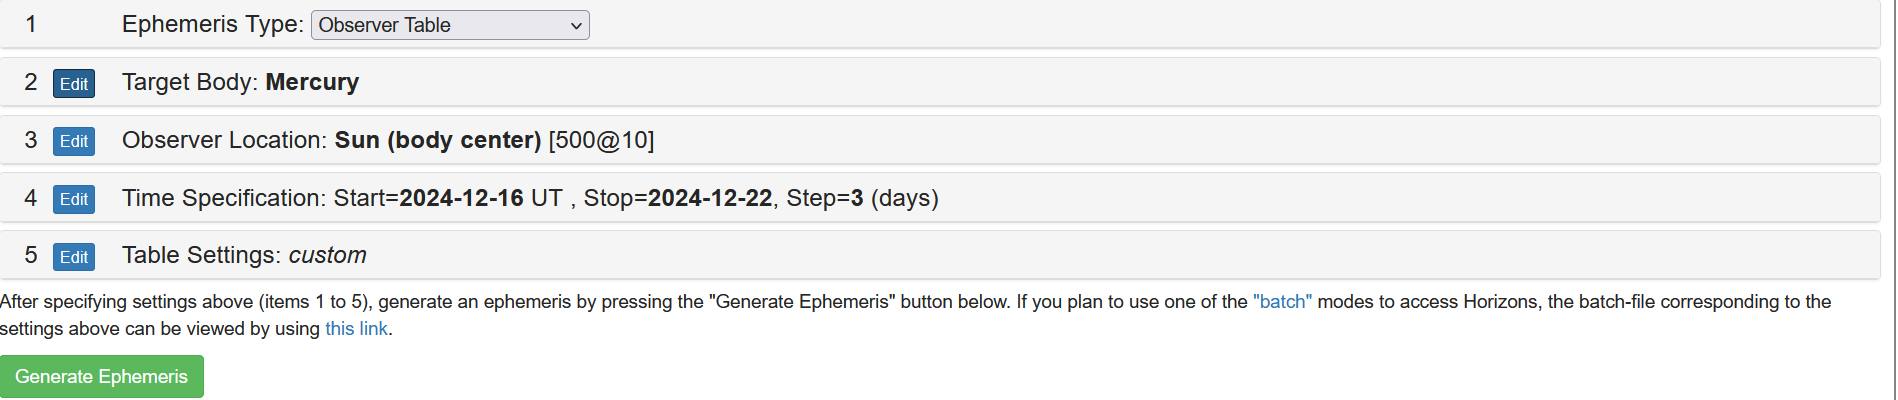
\includegraphics[width=1\textwidth]{b.png}
    \caption{Ilustración de los ajustes seleccionados}
\end{figure}
\newpage
Como vemos, en table pone: Custom. Este es el punto más importante 
ya que a partir de los datos seleccionados de la tabla podremos 
calcular nuestra posición en forma vectorial. Estos datos 
son la latitud heliocéntrica y la longitud heliocéntrica. \\

Una vez le demos a "Generate Ephimeris" obtendremos esos 
valores y podremos obtener las componenetes de nuestro vector 
posición de la siguiente manera. 
\begin{align*}
    &r_{x}=r\cos(\beta)\cos(\lambda) \\
    &r_{y}=r\cos(\beta)\sin(\lambda) \\
    &r_{z}=r\sin(\beta)
\end{align*}
Siendo r el módulo obtenido previamente con la primera herramienta; 
$\beta$ la latitud heliocéntrica y $\lambda$ la longitud heliocéntrica. \\

Con todo esto explicado, ya estamos en disposición de mostrar 
los resultados obtenidos. Cabe recalcar que se han obtenido resultados 
para cada vector de posición. Estos resultados para $\overrightarrow{r_{1}}$ han sido: 
\begin{center}
    \centering
    \begin{tabular}{|c|c|c|c|c|}
    \hline
    $\overrightarrow{v}\, (km/s)$ & $h\, (kg\, km^{2}/s)$ & $i\, (^{\circ})$ & $\Omega\, (^\circ)$ & $e$ \\ \hline
    $(-43,37, -30,07, 2,22)$ & $2,62 \cdot 10^{9}$ & $7,10$ & $54,46$ & $0,17$  \\ \hline
    \end{tabular}
\end{center}

\begin{center}
    \centering
    \begin{tabular}{|c|c|c|c|c|}
    \hline
    $\omega\, (^\circ)$ & $a\, (km)$ & $\theta (^\circ)$ & $r_{p}\, (km)$ & $T\, (dias)$\\ \hline
    $358,37$ & $5,32\cdot 10^{7}$ & $81,17$ & $4,4\cdot 10^{7}$ & $77,31$ \\ \hline
    \end{tabular}
\end{center}
Por su parte, para $\overrightarrow{r_{2}}$ obtuvimos:
\newpage
\begin{center}
    \centering
    \begin{tabular}{|c|c|c|c|c|}
    \hline
    $\overrightarrow{v}\, (km/s)$ & $h\, (kg\, km^{2}/s)$ & $i\, (^{\circ})$ & $\Omega\, (^\circ)$ & $e$ \\ \hline
    $(-32,91, -38,31, -0,78)$ & $2,62 \cdot 10^{9}$ & $7,19$ & $42,32$ & $0,17$  \\ \hline
    \end{tabular}
\end{center}

\begin{center}
    \centering
    \begin{tabular}{|c|c|c|c|c|}
    \hline
    $\omega\, (^\circ)$ & $a\, (km)$ & $\theta (^\circ)$ & $r_{p}\, (km)$ & $T\, (dias)$\\ \hline
    $10,41$ & $5,32\cdot 10^{7}$ & $96,72$ & $4,4\cdot 10^{7}$ & $77,41$ \\ \hline
    \end{tabular}
\end{center}
Mientras que para $\overrightarrow{r_{3}}$ obtuvimos:

\begin{center}
    \centering
    \begin{tabular}{|c|c|c|c|c|}
    \hline
    $\overrightarrow{v}\, (km/s)$ & $h\, (kg\, km^{2}/s)$ & $i\, (^{\circ})$ & $\Omega\, (^\circ)$ & $e$ \\ \hline
    $(-20,42, -43,00, -3,54)$ & $2,58 \cdot 10^{9}$ & $7,90$ & $32,21$ & $0,18$  \\ \hline
    \end{tabular}
\end{center}

\begin{center}
    \centering
    \begin{tabular}{|c|c|c|c|c|}
    \hline
    $\omega\, (^\circ)$ & $a\, (km)$ & $\theta (^\circ)$ & $r_{p}\, (km)$ & $T\, (dias)$\\ \hline
    $13,72$ & $5,17\cdot 10^{7}$ & $118,97$ & $4,2\cdot 10^{7}$ & $74,10$ \\ \hline
    \end{tabular}
\end{center} 
Como era de esperar, los valores de los elementos orbitales 
que se han obtenido con cada medida son muy similares entre sí, excepto 
en aquellos como $\theta$ en los que su valor depende directamente de 
la posición de nuestro cuerpo celeste. 
El único que difiere un poco de las otras dos es la tercera medida. 
La posible causa de esto junto con un tratamiento de errores 
se hará en la siguiente sección. 
\subsection{Método de Gauss}
\section{Conclusiones} %A lo mejor podemos anañizar los resultados aquí
\index{Conclusiones}
El objetivo principal de esta sección es hacer un análisis 
de errores a los datos mostrados en el apartado anterior y, 
a partir de eso, sacar las conclusiones pertinentes. 
\subsection{Método de Gibbs}
Vamos a empezar mostrando los valores de los elementos orbitales 
de la órbita de Mercurio de la literatura: 
\begin{center}
    \centering
    \begin{tabular}{|c|c|c|c|c|c|}
    \hline
    $\overline{v}\, (km/s)$ & $h\, (kg\, km^{2}/s)$ & $i\, (^{\circ})$ & $a\, (km)$ & $e$ & $T\, (dias)$ \\ \hline
    $47,87$ & $2,71 \cdot 10^{9}$ & $7,005$ & $5,791\cdot 10^{7}$ & $0,2056$ & $87,97$ \\ \hline
    \end{tabular}
\end{center}

\subsection{Método de Gauss}
\subsection{Comparación del método de Gibbs y el método de 
Gauss}
\end{document}